\documentclass[12pt]{article}
\usepackage[english]{babel}
\usepackage[utf8x]{inputenc}
\usepackage[T1]{fontenc}
\usepackage{float}
\usepackage{scribe}
\usepackage{listings}

\Scribe{Group 19, Group 20}
\Lecturer{Abir De}
\LectureNumber{10}
\LectureDate{8th September 2022}
\LectureTitle{Introduction to Classification using SVM}

\lstset{style=mystyle}

\begin{document}
	\MakeScribeTop

%#############################################################
%#############################################################
%#############################################################
%#############################################################


%% ##### Small roundup of Lecture ########
We begin by defining the classification problem and then introduce a linear classifier with a bias. We work on ways to find the appropriate parameters for such a model. For a slightly complex and more realistic classification problem, we progress towards the commonly used \textit{hinge-loss} function for SVM.

\section{Introduction}
We now introduce the classification problem. Our dataset will be of the form $\mathbb{D}=\{(x_i,y_i)\}_{i=1}^N$. Similar to regression, the $x_i$ are data points, usually in $\mathbb{R}^k$ for some $k \in \mathbb{N}$. But unlike regression, $y_i$s are now discrete. For a 2 class problem, the set of possible labels can be \{+1,-1\}, \{Cat,Dog\} etc. Even if they are written as \{+1,-1\}, for the purpose of a classification problem we shall always assume there is no partial order among the labels.\\[2mm]
\textbf{Note-} Take a \textit{ranking} task where all objects are given labels from \{1,2,3,4,5\}. These labels are assumed to posses an implicit partial order. This task can thus use this ordering information and is different from our classification problem. In fact, this is called \textit{ordinal regression}.\\[2mm]
Let us consider 2 dimensional data points with class labels from \{+1,-1\} as shown below\\
%\textbf{\textcolor{red}{insert fig}}\\

 \begin{figure}[H]
    \centering
    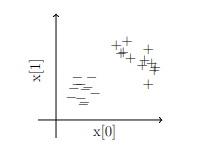
\includegraphics[width=6.5cm]{clusters.png}
    \caption{Cluster of positive and negative labels}
\end{figure}

A few simple classifiers are listed below :
\begin{itemize}
    \item \textbf{Constant model classifier}:- Such a classifier will assign a constant label to every data point. Clearly, if samples from multiple labels are present in the test dataset, it is impossible for a constant model to produce a zero error - even on the training dataset.
    \item \textbf{Unsupervised classifier}:- Unsupervised classifier perform no learning and use heuristics to assign a label to a test data point. For example, an unclassified classifier can find the closest point to the test point in the training dataset and return the class label of this point. Another approach might involve calculating the centroid of all class labels and return the label of the class whose centroid lies closest to the test point. Such models have limited utility.
\end{itemize}
Supervised learning solutions to the problem follow :
\section{Linear Classifier}
One way to define a classifier is to introduce a parameter $w \in \mathbb{R}^k$. Then,
$$\mathbf{w}^Tx > 0 \; \Rightarrow \; y=+1$$
$$\mathbf{w}^Tx < 0 \; \Rightarrow \; y=-1$$
A classifier of this form will fail to provide a significant margin between the classes. To counter this issue, we change the classification rules to the following :
$$\mathbf{w}^Tx > +1 \; \Rightarrow \; y=+1$$
$$\mathbf{w}^Tx < -1 \; \Rightarrow \; y=-1$$
You might ask how one came up with the magic numbers +1 and -1? These numbers don't matter as $w$ can be scaled appropriately to get the exact same classifier whatever $\{-\delta, +\delta\}$ pair one choses to set the margins.\\[2mm]
A major problem with the current classifier is that the origin is never classified to any class label. This is unnecessarily restrictive. For example, consider the following dataset which cannot be seperated by a line passing through the origin but is clearly seperable by a line that does not.
 \begin{figure}[H]
    \centering
    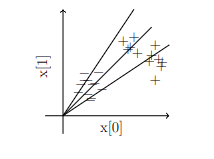
\includegraphics[width=6.5cm]{inseperable-no-bias.png}
    \caption{Angularly inseperable clusters}
\end{figure}
\textbf{Note-} Angularly seperable clusters can be seperated using the current classification model.
 \begin{figure}[H]
    \centering
    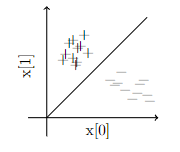
\includegraphics[width=6cm]{angular-seperable.png}%
    \caption{Angularly separated clusters}
\end{figure}

Solving this issue is simple, clearly we are missing a bias term in our rules :
$$\mathbf{w}^Tx + \mathbf{b} > 1 \; \Rightarrow \; y=+1$$
$$\mathbf{w}^Tx + \mathbf{b} < -1 \; \Rightarrow \; y=-1$$
Now, our model has 2 parameters to train, $w,b \in \mathbb{R}^k$. We shall discuss methods of finding a working pair of $w,b$ which are capable of correctly classifying a training dataset.\\[2mm]
A proposed solution is to find 2 points that are closest to one another and lie in different classes and use the perpendicular bisector between this pair as the seperation boundry. Clearly this is a heuristic and a intrinsically unsupervised approach and a counter example can be easily found -
\begin{figure}[H]
    \centering
    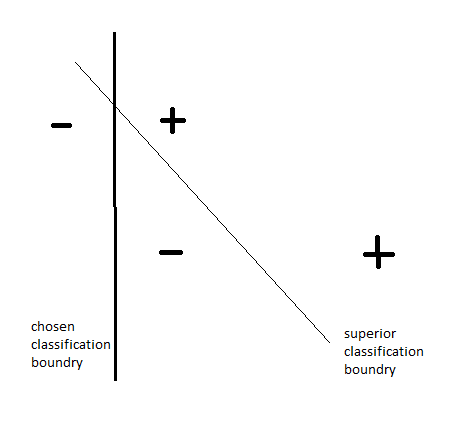
\includegraphics[width=9cm]{counter-perp-bisector.png}%
    \caption{The perpendicular bisector approach does not work.}
\end{figure}
\section{Convex Optimization}
Clearly there can be multiple $w,b$ such that the classifier
$$\mathbf{w}^Tx + \mathbf{b} > +1 \; \Rightarrow \; y=+1$$
$$\mathbf{w}^Tx + \mathbf{b} < -1 \; \Rightarrow \; y=-1$$
classifies the training data reasonably well.\\[2mm] 
The pair of conditions can be rewritten as $ y_i(\mathbf{w}^Tx_i+\mathbf{b}) > 1$ if the class labels are fixed to be $\{+1,-1\}$.\\[1mm] 
Our aim is to find a convex objective function $\mathbf{c}$ for which one can perform : 
$$\{\mathbf{w}^*,\mathbf{b}^*\}=argmin \; \mathbf{c(w,b)} \;\; : \;\; \forall i \in \mathbb{D}\;\; y_i({\mathbf{w}^*}^Tx_i+\mathbf{b}^*) > 1$$
which captures the gist of the problem we are trying to solve. A few proposals follow :
\begin{itemize}
    \item Let the perpendicular distance of the $i^{th}$ positive point from a line $\{\mathbf{w},\mathbf{b}\}$ be $d_i^+(\mathbf{w},\mathbf{b})$ and for the $j^{th}$ negative point be $d_j^-(\mathbf{w},\mathbf{b})$
    $$\mathbf{c(w,b)}:=min_{i\in n_+}\{d_i^+(\mathbf{w},\mathbf{b})\} \cdot min_{j\in n_-}\{d_j^-(\mathbf{w},\mathbf{b})\}$$
    Our optimization problem would have been
    $$\{\mathbf{w}^*,\mathbf{b}^*\}=argmax \; \mathbf{c(w,b)}$$
    We try to maximize this objective function. It is equivalent to minimizing its negative (:\\[1mm]
    This objective function tries to increase the distance of both clusters from our classification line. Convince yourself that a sum would not achieve this 2 fold minimization.\\[1mm]
    This objective function is not easily optimized.
    \item Define 
    $$\mathbf{c(w,b)}=min(min_{i\in n_+}\{d_i^+(\mathbf{w},\mathbf{b})\},min_{ j\in n_-}\{d_j^-(\mathbf{w},\mathbf{b})\})$$ 
    Or
    $$\mathbf{c(w,b)}=min_{\forall i\in \mathbb{D}}\{d_i(\mathbf{w},\mathbf{b})\}$$
    Here, we are interested in maximizing the minimum distance across all points. If this quantity is large, then all other distances will be large.\\
    In fact, perpendicular distance of the $i^{th}$ point from the line $\mathbf{w}^Tx+\mathbf{b}=0$ is given by $d_i=\frac{|\mathbf{w}^Tx_i+\mathbf{b}|}{||\mathbf{w}||}$.\\[1mm] 
    Since this is a constrained minimization (maximization), we have $y_i(\mathbf{w}^Tx_i+\mathbf{b}) > 1$. Thus,
    $$d_i=\frac{|\mathbf{w}^Tx_i+\mathbf{b}|}{||\mathbf{w}||} > \frac{1}{||\mathbf{w}||}$$ 
    For increasing $d_i$ over all i, we increase the lower bound on $d_i$.
    \item This leads to the famous regularized loss : 
    $$\{\mathbf{w}^*,\mathbf{b}^*\}=argmin \; ||\mathbf{w}||^2\;\; : \;\;\forall i \in \mathbb{D}\;\; y_i(\mathbf{w}^Tx_i+\mathbf{b}) > 1$$
\end{itemize}
\section{A more realistic task}
% \textbf{\textcolor{red}{insert fig}}\\
After seeing how to select a good classifier when multiple are available, it is time to look at a more real world problem. Clearly the set of inequalities 
$$\forall i \in \mathbb{D}\;\; y_i({\mathbf{w}^*}^Tx_i+\mathbf{b}^*) > 1$$
need not always have a $\mathbf{w,b}$ pair satisfying them. Consider the following figure :
\begin{figure}[H]
    \centering
    \includegraphics[width=6cm]{overlapping-clusters.png}
    \caption{Overlapping clusters. The points cannot be linearly classified.}
\end{figure}
Dropping constraints, one can simultaneously minimize $\mathbf{c}$ and the missclassification count :
$$|\{i\; : \;|y_i(\mathbf{w}^Tx_i+\mathbf{b})|\leq 1\}|$$
However, this doesn't take into consideration the degree of misclassification. The points for which $|y_i(\mathbf{w}^Tx_i+\mathbf{b})|\sim 1$ are treated the same as the points for which $|y_i(\mathbf{w}^Tx_i+\mathbf{b})|\sim 0$. To counter this, we introduce the hinge loss over $y_i(\mathbf{w}^Tx_i+\mathbf{b})-1$ and use it to train the SVM.\\
The final loss function looks like :
$$ \mathbf{w}^*, \mathbf{b}^* = argmin_{w,b} \sum_i H(y_i(\mathbf{w}^Tx_i+\mathbf{b})-1) + \lambda||w||^2 $$

\end{document}